\section{Exercise 04: SQL Injection}

\subsection{SQL Injection}

\subsubsection{Does it mean the MySQL server is protected against cyber attacks? From Kali, try:mysql -h <METASPLOITABLE IP> -P 3306}
Not necessarily. Restricting version enumeration is just one security measure. There could
be other vulnerabilities, misconfigurations, or security flaws still present.

\begin{figure}[H]
      \centering
      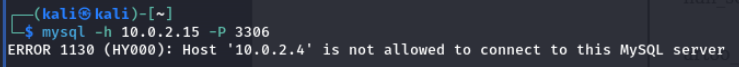
\includegraphics[width=0.8\linewidth]{pic/mysql.png}
      \caption{mysql}
      \label{fig:mysql}
\end{figure}


\subsubsection{How could that protection look like?}
The protection might involve configurations that restrict information disclosure to
unauthenticated users. This can be achieved through configurations in the MySQL server
settings. It might also involve a firewall or Intrusion Prevention System (IPS) that detects and
blocks such probes.

\subsubsection{And what exactly would it protect against?}
Hiding the version number primarily protects against version-specific attacks. If an attacker
doesn't know the version, they might have a harder time determining which exploits might
work against that specific version. However, this won't stop determined attackers who might
use other methods to determine the version or who might attempt to exploit the server
blindly.



\subsection{Spying with SQL Injection}

\subsubsection{Please shortly discuss your opinion of this web servers configuration concerning directly listings.}
Directory listing should never  be enabled for websites that are open to the public. because revealing the
directory structure can give attackers insights into potential security problems, hidden files, or
backup files that might be exploited.


\subsubsection{What type of SQLi attack works? Can you explain why?}
The attack you're attempting is called a Boolean-based blind SQL injection. When you input
conditions like \textit{‘ OR 1=1;} if the system is vulnerable, it takes your input and constructs a
query that always evaluates to true because 1=1 is a universally true condition. This typically
works on systems where inputs are not sanitized or parameterized. In the absence of proper
input validation, the raw input gets directly placed into the SQL query, leading to the injection
attack.
When running the \textit{‘ OR 1=1;} for instance when we go the IP though the webpage
10.0.2.15 and we will see an login page

\begin{figure}[H]
      \centering
      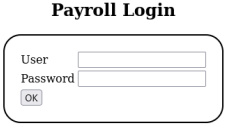
\includegraphics[width=0.3\linewidth]{pic/payroll.png}
      \caption{payroll}
      \label{fig:payroll}
\end{figure}

From here with we can see that \textit{‘ OR 1=1;} will give us some of the information that's in the
database.

\begin{figure}[H]
      \centering
      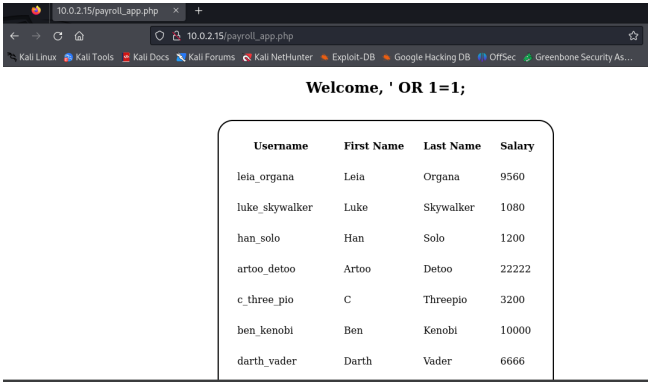
\includegraphics[width=\linewidth]{pic/payroll website.png}
      \caption{payroll website}
      \label{fig:payroll website}
\end{figure}


\subsubsection{What is the \# sign for? Can we generally assume it to do the trick?}
The \textit{\#} sign is used to comment out the rest of the SQL query. By including it, you're
ensuring that whatever follows your injection will be ignored. In MySQL, the \textit{\#} is a
single-line comment symbol. While it often works in the context of SQL injections against
MySQL databases, other databases use different comment symbols (like ‘--’ for SQL
Server). So, you cannot universally assume \textit{\#} will always work; it's specific to the database
in use.


\subsubsection{Include four relevant username/password combinations in your report. What is the issue with the passwords in the data base and what could bedone to secure them?}
One significant issue with password storage in databases is the potential storage of passwords in plaintext.
This makes them easily accessible in the event of a database breach. To enhance password security,
the following measures should be implemented:

\begin{itemize}
      \item \textbf{Hash Passwords:} Utilize strong cryptographic hash functions, such as bcrypt or Argon2, to store password hashes rather than plaintext passwords. This conversion makes it significantly more challenging for attackers to decipher the actual passwords.
      \item \textbf{Use Salts:} Integrate passwords with a unique, random value known as a \textit{salt} before hashing. This process ensures that identical passwords will generate different hash values, further complicating attempts at unauthorized access.
      \item \textbf{Implement Strong Password Policies:} Establish policies that mandate long, complex passwords. This strategy helps to prevent brute-force attacks by significantly increasing the difficulty and time required to crack passwords.
\end{itemize}

Ensuring robust password security is crucial for protecting sensitive data and maintaining overall system integrity.

\begin{figure}[H]
      \centering
      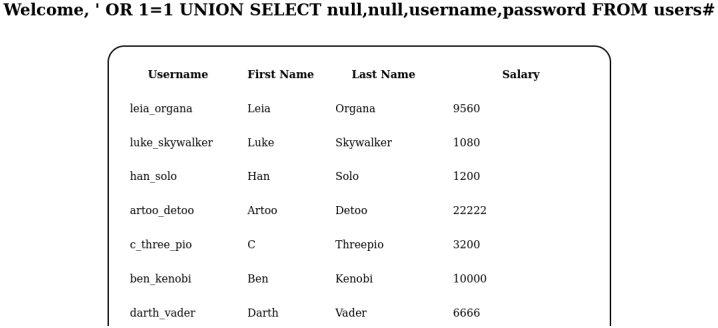
\includegraphics[width=\linewidth]{pic/username and password 1.png}
      \caption{username and password 1}
      \label{fig:username and password 1}
\end{figure}

\begin{figure}[H]
      \centering
      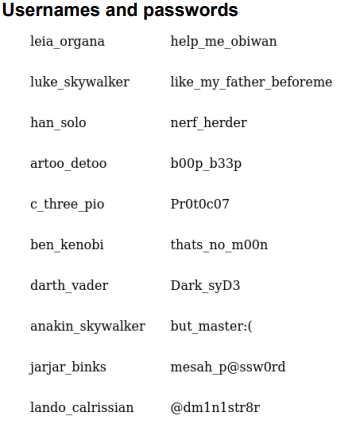
\includegraphics[width=0.4\linewidth]{pic/username and password 2.png}
      \caption{username and password 2}
      \label{fig:username and password 2}
\end{figure}


\subsubsection{Which other problem allows you to get into the machine using ssh? Howcould this be prevented?}
The issue at hand is twofold:

\begin{itemize}
      \item \textbf{Weak Passwords:} The use of weak passwords for system authentication poses a significant risk. Such passwords can be easily brute-forced or guessed by attackers, especially if they are already known or exposed.

      \item \textbf{SSH Access:} Currently, SSH access to the machine is unrestricted. Coupled with the exposure of credentials, this becomes a critical vulnerability.
\end{itemize}

\subsection*{Preventive Measures for Unauthorized SSH Access}
To enhance security and prevent unauthorized SSH access, the following strategies should be adopted:

\begin{itemize}
      \item \textbf{Use Key-Based Authentication:} Opt for cryptographic SSH keys over password-based authentication. This approach is significantly more secure.

      \item \textbf{Restrict SSH Access:} Limit SSH access to specific IP addresses or networks. This control measure greatly reduces the potential for unauthorized access.

      \item \textbf{Implement Fail2Ban or Similar:} Use tools like Fail2Ban to automatically block IP addresses that exhibit malicious activities, such as numerous password failures.

      \item \textbf{Change the Default SSH Port:} Altering the default port (22) for SSH can help deter automated attacks. Though this is a form of security through obscurity, it can be an effective measure in reducing unsophisticated attacks.
\end{itemize}

\textit{Example Scenario:} Executing the command \textit{ssh leia\_organa@10.0.2.15} prompts a login option. Possessing the pre-known password allows for system access under this scenario.

\begin{figure}[H]
      \centering
      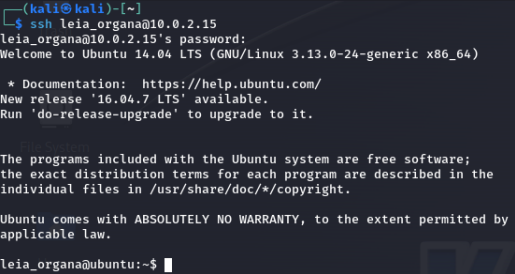
\includegraphics[width=0.8\linewidth]{pic/ssh leia_organa@10.0.2.15.png}
      \caption{ssh leia\_organa\@10.0.2.15}
      \label{fig:ssh leia_organa@10.0.2.15}
\end{figure}

By running \textit{groups} we can see that the user has root access, which means so do we since
we have the login information for the user.


\begin{figure}[H]
      \centering
      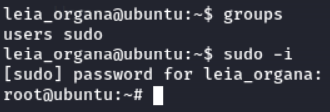
\includegraphics[width=0.4\linewidth]{pic/leia_organa.png}
      \caption{leia\_organa}
      \label{fig:leia_organa}
\end{figure}








\subsection{Elevation of Privilege}

\subsubsection{Which are the individual issues that allowed us to go from a web interfaceto root access, and how would you address them as a servers operator toprevent them being exploited? Describe the issues you identified and tryto come up with suggestions on how to fix them.}
\begin{itemize}
      \item \textbf{SQL Injection Vulnerability:}
            The web interface did not validate or sanitize input, allowing for SQL injection.
            \begin{itemize}
                  \item Fix: Use prepared statements and parameterized queries. Validate and sanitize all user inputs.
            \end{itemize}

      \item \textbf{Exposed Usernames and Passwords:}
            The database contained plaintext passwords, allowing for direct access to the system.
            \begin{itemize}
                  \item Fix: Store passwords as salted hashes using strong cryptographic algorithms. Regularly audit and monitor database access.
            \end{itemize}

      \item \textbf{Weak System Passwords:}
            The exposed passwords were also used for system authentication.
            \begin{itemize}
                  \item Fix: Use strong, unique passwords for every system/service. Implement multi-factor authentication where possible.
            \end{itemize}

      \item \textbf{Elevated Privileges:}
            The compromised users had sudo or wheel group permissions, allowing for privilege escalation.
            \begin{itemize}
                  \item Fix: Follow the principle of least privilege. Only grant users the minimum necessary permissions.
            \end{itemize}

      \item \textbf{Unrestricted SSH Access:}
            The system allowed SSH access without restrictions.
            \begin{itemize}
                  \item Fix: Limit SSH access to specific IP addresses, use key-based authentication, and implement tools like Fail2Ban.
            \end{itemize}
\end{itemize}




\subsubsection{Can SQL Injection expose an otherwise inaccessible data base server?}
Yes, SQL injection can be used to expose and retrieve data from a database that might not
be directly accessible from the outside. If an application interfaces with that database and is
vulnerable to SQL injection, an attacker can manipulate the application's SQL queries to
retrieve, modify, or delete data, even if the database itself is not directly exposed to the
internet.


\subsubsection{How likely do you think an attack scenario as presented here is?}
This scenario, while somewhat rare and this is for a teaching purposes, it represents a real and
prevalent risk. Such vulnerabilities do still exist, and there have been numerous
instances of companies and platforms being compromised due to similar vulnerabilities and
misconfigurations but they are becoming rare. The probability of this exact sequence of vulnerabilities existing on a
well-maintained and updated system is lower, but even one of these vulnerabilities can lead
to significant compromises. Proper system hardening, regular security audits, and
continuous monitoring can mitigate such risks.

\subsection{Using our Foot in the Door for Access to Other Services}

\subsubsection{Is sudo necessary? What do we gain by using it?}
In this context, where you already have root access, the use of sudo is redundant. When
youre operating as the root user, you have superuser permissions, so using sudo
is not necessary. The sudo command is typically used to grant elevated permissions to a
regular (non-root) user for specific tasks. By using it, you can execute certain commands as
the superuser or another user, as specified by the security policy.
The primary gain of using sudo in regular scenarios (not as root) is that it provides a
mechanism to delegate authority. It allows a permitted user to execute a command as the
superuser or another user, as specified in the /etc/sudoers file. It's a way of giving certain
users the ability to run some or all commands as root without having to know the root
password.


\subsubsection{Are there other ways to search for a file? Which do you know?}
\begin{figure}[H]
      \centering
      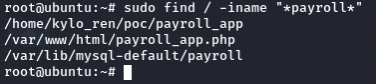
\includegraphics[width=0.6\linewidth]{pic/sudo find.png}
      \caption{sudo find}
      \label{fig:sudo find}
\end{figure}

Yes there is multiple ways to search for a file in Linux examples given below:

\textbf{Using locate}
This command uses a prebuilt database of files to search. It's often faster than find
but may not have the most up-to-date information.

\textit{locate payroll}

\textbf{Using grep}
While grep is primarily used for searching text within files, you can use it in
combination with other commands to find files. For example, you can use grep with ls
to search within a specific directory:

\textit{ls /path/to/directory | grep "payroll"}

\textbf{Using which}
This command is used to locate executable files in system directories.
which payroll

\textbf{Using whereis}
This command helps to locate the binary, source, and manual page files for a
command.

\textit{whereis payroll}


\subsubsection{Can you find anything interesting?}
First we use the following command:

\textit{cd /var/www/html/}

Then we do cat into the .php file and we get the following below:

\textit{cat payroll\_app.php}

\begin{figure}[H]
      \centering
      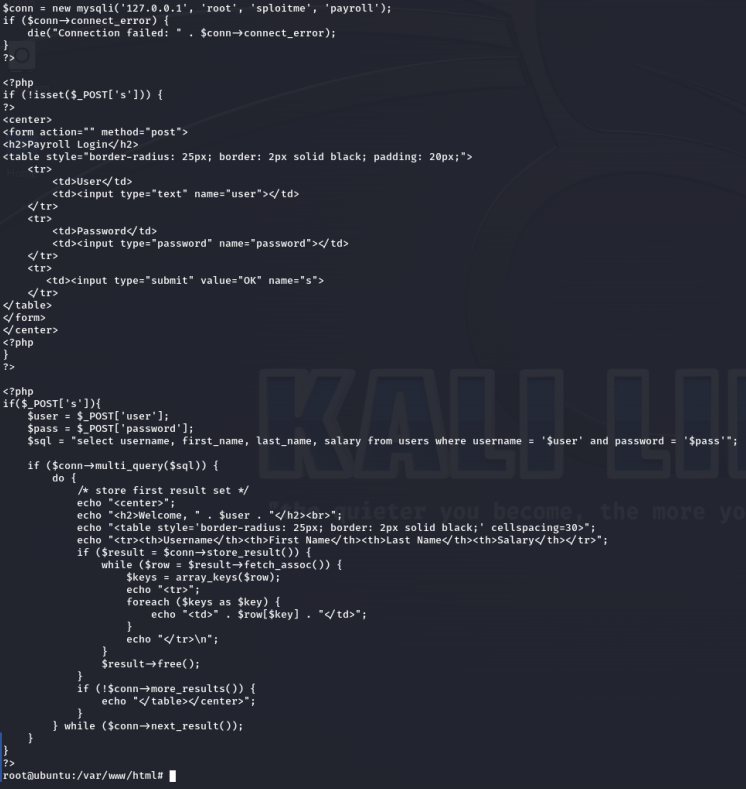
\includegraphics[width=\linewidth]{pic/cat payroll_app.png}
      \caption{cat payroll\_app}
      \label{fig:cat payroll_app}
\end{figure}

With the password to the database we can now enter it can see what it contains with the
following command:

\textit{mysql -h 127.0.0.1 -P 3306 -u root -p}

We know the password from beforehand: sploitme

Here we can look into what data there is stored for this instance there are users stored and
with the following command we can see the table:

\textit{select * from users;}

\begin{figure}[H]
      \centering
      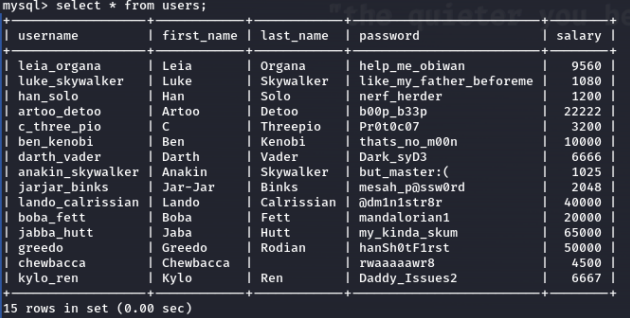
\includegraphics[width=0.8\linewidth]{pic/select from users;.png}
      \caption{select from users;}
      \label{fig:select from users;}
\end{figure}


\subsubsection{Whats the user name, password and database name?}

\begin{figure}[H]
      \centering
      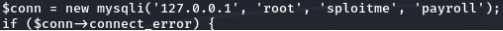
\includegraphics[width=0.8\linewidth]{pic/database info.png}
      \caption{database info}
      \label{fig:database info}
\end{figure}

\textbf{User name:} root

\textbf{Password:} sploitme

\textbf{Database name:} payroll


\subsubsection{What was the problem with the web application?}
The web application was vulnerable to SQL injection attacks because of its insecure method
of handling user inputs. It used string concatenation to create SQL statements directly from
user inputs without any form of validation or sanitization. This allowed for malicious SQL
statements to be executed, granting unauthorized access to the database.


\subsubsection{Which ports and services were the problem associated with?}
The problems were associated with the HTTP service on port 80 (where the web application
was running) and the MySQL service on port 3306.


\subsubsection{How did you exploit the vulnerability?}
The vulnerability was exploited by inserting SQL statements into the input fields of the web
application. By appending malicious SQL logic (such as \textit{' OR 1=1;}), it was possible to
manipulate the SQL query to the application's detriment.


\subsubsection{And what were you able to do?}
Once the SQL injection vulnerability was exploited, unauthorized access to user details
including usernames and passwords from the database was gotten. With this information,
we could gain SSH access to the machine and root access. also, by analyzing the
PHP code, the database connection details were extracted, granting full database access.

\subsubsection{How would you suggest to fix the problem? (Do some online research aboutSQL injections solutions.)}
To enhance the security of the application and protect against SQL injection attacks, the following measures should be implemented:

\begin{itemize}
      \item \textbf{Use Prepared Statements or Parameterized Queries:} This approach ensures that user inputs are always treated as data, not as executable code.

      \item \textbf{Implement Input Validation:} Validate all user-submitted data against specific patterns or ranges to prevent malicious input.

      \item \textbf{Utilize Web Application Firewalls (WAFs):} WAFs are effective in detecting and blocking SQL injection attempts.

      \item \textbf{Limit Database User Privileges:} Avoid using accounts like "root" or "admin" for database connections. Opt for accounts with the least privileges necessary for the required operations.

      \item \textbf{Regularly Update and Patch Software Components:} Keeping software up-to-date is crucial in mitigating vulnerabilities that can be exploited via SQL injection.

      \item \textbf{Educate Developers:} Inform and train developers in secure coding practices to build a strong first line of defense against injection attacks.
\end{itemize}

\subsubsection{Draft a shortly and crisply, the relevant parts of a policy trying to prevent theseissues.}
\textbf{Purpose:}
To safeguard our organization's data and applications from unauthorized access and potential security breaches.

\textbf{Scope:}
This policy applies to all developers, IT staff, and any third parties developing applications on behalf of the organization.

\textbf{Policy:}
\begin{itemize}
      \item Database queries must be executed using prepared statements or parameterized queries.
      \item User inputs must undergo strict validation and sanitization before use.
      \item Database connections should be established with the least privileged user.
      \item Regularly audit and update systems to patch vulnerabilities.
      \item Employ a web application firewall (WAF) to monitor, alert, and block malicious queries.
      \item Staff must undergo periodic security training to stay updated with the latest threats and prevention techniques.
\end{itemize}

\textbf{Enforcement:}
Any developer or third party found in violation of this policy may face disciplinary actions, up to and including termination.

\subsection{Fully Explore Local Accounts}

\subsubsection{What are benefits of performing this scan after already having full access?}
Performing a password-cracking operation, even when full system access has already been obtained, can offer several advantages:

\begin{itemize}
      \item \textbf{Expanding Access:}
            Accessing different user accounts can grant permissions or access to specific data not available to the current user or even the root account.

      \item \textbf{Pivot to Other Systems:}
            Since users often reuse passwords, cracking local passwords may enable access to additional systems, applications, or network segments using the same credentials.

      \item \textbf{Understanding Security Posture:}
            The ease of cracking local passwords can reveal insights about the organization's password policies, highlighting potential weaknesses.

      \item \textbf{Maintaining Persistent Access:}
            Possessing credentials for multiple accounts can be crucial for retaining access over time, especially if root access is later compromised or revoked.

      \item \textbf{Avoiding Detection:}
            Performing actions as a regular user might be less conspicuous than using a root or admin account, which could be more likely to trigger security alerts.

      \item \textbf{Credential Gathering for Reporting:}
            In ethical hacking or penetration testing, gathering comprehensive data is essential. Demonstrating the ability to crack local passwords provides critical feedback for clients, underscoring vulnerabilities that need addressing.
\end{itemize}

Despite having the highest level of access, delving further into password cracking can uncover more covert access routes, provide insights into security practices, and enhance the thoroughness of penetration test reporting.




\subsection{Post-Exploitation}

\subsubsection{Thinking as an attacker, what would your next steps be?}

\begin{enumerate}
      \item \textbf{Persistence:}
            Establish multiple backdoors to maintain access to the system, even if one entry point is detected and closed.

      \item \textbf{Data Exfiltration:}
            Identify and extract critical data (personal, financial, intellectual property), potentially encrypting it for financial gain, further attacks, or ransom demands.

      \item \textbf{Lateral Movement:}
            Utilize the compromised host as a base for moving within the network, targeting additional systems to expand control.

      \item \textbf{Elevate Privileges:}
            If not operating at the highest privilege level, seek ways to escalate privileges for broader access or control.

      \item \textbf{Scout for More Targets:}
            Employ scanning tools to find other vulnerable systems within or associated with the initial target's network.

      \item \textbf{Establish Command \& Control (C2):}
            Create a channel for remote command execution, updates, or data transfer with the compromised system.

      \item \textbf{Cover Tracks:}
            Clear logs, erase command histories, and use other methods to reduce detection likelihood.

      \item \textbf{Deploy Malware:}
            Depending on the objective, introduce malware such as ransomware, keyloggers, or Trojans to fulfill specific agendas.

      \item \textbf{Monetize the Attack:}
            Profit from the breach by selling system access, employing the system for crypto-mining, or leveraging stolen data.
\end{enumerate}

\subsubsection{As an operator, what would you do to counteract?}
\begin{enumerate}
      \item \textbf{Detection:}
            Implement intrusion detection systems (IDS) and intrusion prevention systems (IPS) to detect and thwart suspicious activities.

      \item \textbf{Incident Response:}
            Mobilize an incident response team to evaluate the breach, comprehend its scope, and devise a recovery strategy.

      \item \textbf{Isolate Affected Systems:}
            Sever the network connection of compromised systems to inhibit further lateral movement or data theft.

      \item \textbf{Backup \& Restore:}
            Utilize clean backups to restore systems to their pre-compromise state.

      \item \textbf{Patch \& Update:}
            Update all systems with the latest security patches, focusing on those compromised.

      \item \textbf{Password Reset:}
            Mandate password changes for all users, especially those with breached accounts.

      \item \textbf{Log Analysis:}
            Scrutinize logs to trace the intruder's activities, entry methods, and impacted data.

      \item \textbf{Enhance Monitoring:}
            Intensify monitoring efforts to spot any recurrence of the attacker or other anomalous activities.

      \item \textbf{User Training:}
            Conduct training for users to aid in the recognition and reporting of suspicious actions or phishing schemes.

      \item \textbf{Regular Audits:}
            Perform consistent security audits and vulnerability scans to uncover and address potential vulnerabilities.

      \item \textbf{Network Segmentation:}
            Segregate crucial assets from the general network to impede lateral attacks.

      \item \textbf{Engage External Experts:}
            In cases of severe breaches, consider hiring external cybersecurity professionals for comprehensive analysis and advice.
\end{enumerate}



\subsection{Obfuscated Malware}

\subsubsection{Task 1 - Take your time to look at the code. Is it readable?}
Given the current state of the script, it's not immediately readable since it's obfuscated using
Base64 encoding.

\subsubsection{Task 2 - The script is Base64 encoded charset UTF-8. You need to decode the
      python script by copying the "jibberish" text that is between the quotes for the
      payload variable. You can use, e.g., base64encode.net or any Base64 decoder
      that you find online.}

\begin{figure}[H]
      \centering
      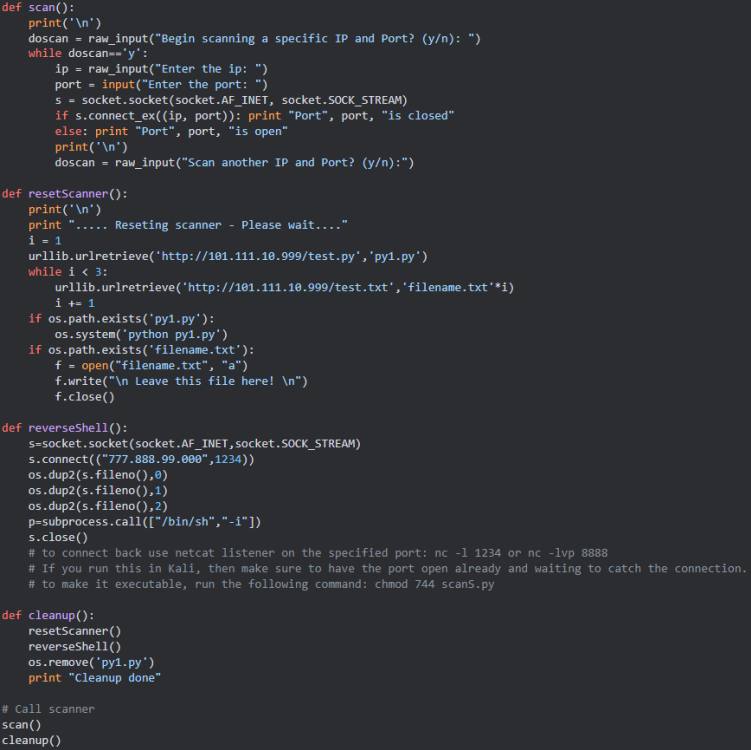
\includegraphics[width=0.9\linewidth]{pic/python script.png}
      \caption{python script}
      \label{fig:python script}
\end{figure}


\subsubsection{Task 3 - What does the code do? Is it a malicious software and if so how wouldyou classify it?}
\begin{itemize}
      \item The \textbf{scan function} is legitimate and performs as indicated by the script's title, it assesses whether specific ports on an IP address are open or closed.

      \item The \textbf{resetScanner function} attempts to download and execute a Python file from a specific IP address, which is likely malicious or a placeholder for this exercise. It also repeatedly tries to fetch a text file, appending its contents if the file already exists.

      \item The \textbf{reverseShell function} is decidedly malicious. It aims to establish a reverse shell connection to an IP address (777.888.99.000) on port 1234. This function could allow an attacker to access the host machine where the script is executed.

      \item The \textbf{cleanup function} invokes both resetScanner and reverseShell before deleting a file named \textit{py1.py}.
\end{itemize}

Given these functionalities, I would say its malicious. It serves as a combination of a Port Scanner and a Reverse Shell, hitting the description of a \textit{Trojan Horse}.


